\section{Case Studies}
\label{sec:casestudies}

The random generation framework presented throughout this work allows us to
write extensible generators in a very concise way.
%
However, this expresiveness comes attached to a perceptible runtime overhead.
%
In this section we evaluate the implicit cost of composing generators using
three real-world case studies.


As we have shown in Section \ref{sec:generators}, the random generation
process we propose in this paper can be seen as having two phases.
%
First, generate random values from the representation types used to specify the
shape of our data; and then we use their algebras to translate them to the
corresponding values of our target data types.
%
In particular, the tranformation step is expected to pattern match repeatedly
against the |InL| and |InR| constructors of the |oplus| operators when
traversing each construction injection.
%
Because of this, in general we expect a performance impact with respect to
manually-written concrete generators.


As recently analyzed by \citeauthor{KiriyamaOptimizingDTC}, this slowdown is
expected to be linear in the depth of our representation type
\cite{KiriyamaOptimizingDTC}.
%
Hence, one can drastically reduce the runtime overhead by associating each
|oplus| operator in a balanced fashion.
%
So, for instance, instead of writing |(f oplus'' g oplus'' h oplus'' i)|, which
is implicitly parsed as |(f oplus'' (g oplus'' (h oplus'' i)))|; we can
associate constructions as |((f oplus'' g) oplus'' (h oplus'' i))|, thus
reducing the depth of our representation from four to three levels and, in
general, from a $\mathcal{O}(n)$ to a $\mathcal{O}(log(n))$ complexity in the
runtime overhead, where $n$ is the amount of constructions under consideration.



To evaluate our approach, we analyzed the performance of generating random
values using three real-world case studies:
\begin{inparaenum}[(i)]
\item Red-Black Trees, inspired by Okasaki's formulation,
\item Lisp S-expressions, inspired by the package \emph{hs-zuramaru}, and
\item HTML expressions, inspired by the \emph{html} package, and following the
  same structure as our motivating |Html| example.
\end{inparaenum}
%
The expanse of each case study can be summarized as follows:

\begin{table}[H]
  \begin{tabular}{||c||c||c||c||c||}
    \hline
    Case Study & |Con|s & |Pat|s & |Fun|s & Total Constructions \\ \hline
    \hline
    RBT        & 2      & 6      & 5      & 13                  \\ \hline
    SExp       & 6      & 9      & -      & 15                  \\ \hline
    HTML       & 4      & -      & 132    & 136                 \\ \hline
  \end{tabular}
\end{table}

We benchmarked the execution time required to generate and fully evaluate 1000
random values corresponding to each case study, comparing both manually-written
concrete generators and modular generators obtained using our approach.
%
For this purpose, we used the \emph{Criterion} benchmarking tool for Haskell,
and limited the maximum depth of the generated values to five levels.
%
Additionally, our modular generators were tested using both linear and balanced
generation specifications.
%
Figure \ref{fig:times} illustrates the relative execution time of each case
study, with respect to each manually-written random generator---we encourage the
reader to obtain a colored version of this work.

\begin{figure}[b]
  \centering
  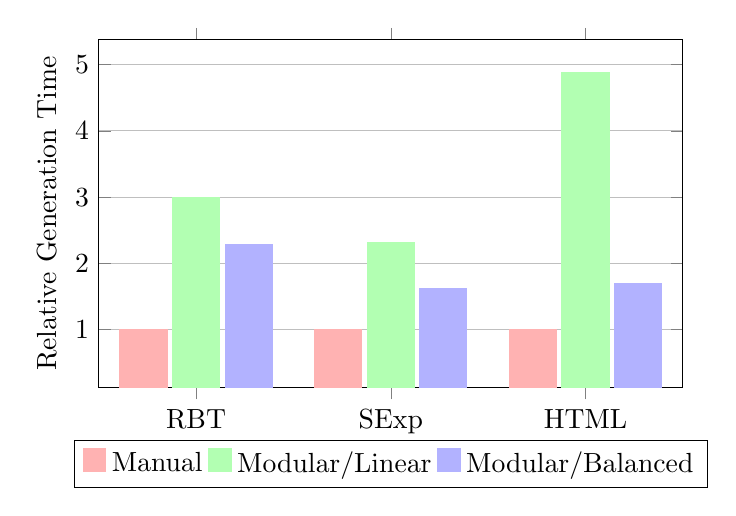
\begin{tikzpicture}
    \begin{axis}
      [ height=6cm
      , width=9cm
      , ybar
      , ymajorgrids=true
      , ytick={0,1,...,5}
      , ymax=4.5
      , enlargelimits=0.25
      , enlarge x limits=0.25
      , /pgf/bar width=17pt
      , legend style={
        at={(0.5,-0.15)},
        anchor=north,legend columns=3}
      , legend image code/.code={%
        \draw[#1, draw=none] (0cm,-0.1cm) rectangle (0.3cm,0.2cm); }
      , ylabel={Relative Generation Time}
      , symbolic x coords={RBT, SExp, HTML}
      , xtick=data
      % , nodes near coords
      , nodes near coords align={vertical}
      ]
      \addplot[fill, red!30]   coordinates {(SExp,1)    (RBT,1)    (HTML,1)};
      \addplot[fill, green!30] coordinates {(SExp,2.31) (RBT,3)    (HTML,4.88)};
      \addplot[fill, blue!30]  coordinates {(SExp,1.62) (RBT,2.28) (HTML,1.70)};
      \legend{Manual, Modular/Linear, Modular/Balanced}
    \end{axis}
  \end{tikzpicture}
  \caption{Generation time comparison between concrete and modular generators.}
  \label{fig:times}
\end{figure}

As it can be observed, our approach suffers from a noticeable runtime overhead,
specially when considering the HTML case study with a large amount of
construction involved at the generation process.
%
However, by balancing our representation types we found that the generation
performance gets dramatically improved.
%
To apply this optimization automatically, and relying on more sophisticated
techniques like prefix-free encodings to obtain optimal representations, is a
undergoing path of our future work.


On the other hand, it has been argued that the generation time is often not
substantial with respect to the rest of the testing process, especially when
testing complex properties over monadic code, as well as using randomly
generated values for penetration testing.


Nonetheless, we consider that these results are in turn very encouraging, given
that the flexibility obtained from using our approach does not produce severe
slowdowns in practice, nor explodes more than linearly as we increase the
complexity of our random generators.
